

	\chapter{Orientation tuning in the Tree Shrew superior colliculus}

	\pagebreak
	\section{Summary}
	
	Though earlier theories of orientation selectivity suggested that orientation biases observed in V1 inputs are the result of excitatory convergence, studies have shown that these biases may be inherited from neurons in sub-cortical structures, namely the lateral geniculate nucleus (dLGN) and ultimately the retina. However, there is some controversy as to whether the biases reported in these sub-cortical structures arise from cortical feedback instead of biased inputs. If orientation selectivity arises from the retina, it should be evident in other targets of retinal projections. The superior colliculus (SC) is one such area. Here, orientation selectivity of SC neurons in tree shrews was measured using thin bars and gratings of different spatial frequencies. SC neurons showed orientation tuning and spatial frequency tuning comparable to that observed in the LGN of tree shrews. At higher spatial frequencies, the orientation selectivity was more evident, similar to that reported in the retina and LGN of cats and macaques. Similar results have also been reported in layer 4 of the tree shrews earlier in this thesis (see Chapter 5). These results indicate that the potential source of orientation biases in the LGN and the SC could be the retina. Direction selectivity and linearity of the SC neurons were also studied.
	
	\pagebreak
	
	
	\section{Introduction}
	
The tree shrew superior colliculus (SC) is a large well laminated structure (Tigges \& Shanta, 1969; Zhou et al., 2016). It is sub-divided into areas important for visual form processing and visuomotor processing (Casagrande et al., 1972; Casagrande \& Diamond, 1974) and has been implicated in an alternative pathway to the visual cortices (Killackey et al., 1971; Killackey \& Diamond., 1971). While the functional role and the projections of the SC have been extensively studied, few studies have characterised the receptive field properties of individual neurons. In this chapter, the receptive field properties, specifically orientation and spatial frequency tuning of the tree shrew SC neurons were studied and compared with the properties of the geniculo-striate system of the tree shrews.
 
Due to its extensive reciprocal projections to sensory as well as motor areas of the brain, the SC was implicated in oculomotor behaviour (Sherrington, 1947). However, studies where different layers of the SC were lesioned showed that the SC consisted of two separate functional systems --- the superficial layers essential for visual form discrimination and the inferior layers implicated in oculomotor function and orienting behaviour (Casagrande et al., 1972; Casagrande \& Diamond, 1974). The superficial layers of the tree shrew SC are further divided into stratum zonale (SZ), stratum griseum superficiale (SGS) and stratum opticum (SO) with the SGS further subdivided into upper and lower SGS (uSGS and lSGS respectively). As these are the layers of the SC that predominantly receive visual input (from the retina and primary visual cortex (V1); see May, 2006 for review), only the response properties of neurons in these superficial layers were studied.

In the present study, we aimed to examine orientation biases in the tree shrew SC. More than 50 years after its first report, the mechanism underlying orientation selectivity is still debated (Ferster \& Miller, 2000; Priebe \& Ferster, 2008; Scholl et al., 2013; Vidyasagar \& Eysel, 2015; Kremkow et al., 2016). The model of excitatory convergence proposed by Hubel \& Wiesel (1962, 1968) for orientation selectivity in cats and macaques assumed that orientation selectivity was first generated in the primary visual cortex along the visual pathway. A similar mechanism, where orientation selectivity is generated for the first time in layer 2/3 of the primary visual cortex has been proposed in the tree shrews (Chisum et al., 2003; Mooser et al., 2004) These theories have largely ignored the orientation biases that have been demonstrated in sub-cortical areas. Subcortical orientation biases have been reported in the retina and the dLGN of most species (cats- Levick \& Thibos, 1980; Vidyasagar \& Urbas, 1982; Levick \& Thibos, 1982; Shou \& Leventhal, 1989; macaques- Smith et al., 1991; Xu et al., 2002, Passaglia et al., 2002; tree shrews- Van Hooser et al., 2013; rodent- Tan et al., 2011; Sun et al., 2016). However, oriented neurons in the superior colliculus have only been reported in rodents (Wang et al., 2010; Inayat et al., 2015; Ahmadlou et al., 2015; Shi et al., 2017). In cats and macaques, direction selectivity has been reported in the Superior Colliculus (McIlwain \& Buser, 1967; Sterling \& Wickelgren, 1969; Rosenquist \& Palmer, 1971; Cynader \& Berman, 1972; Goldberg \& Wurtz, 1972), but units can be selective to direction without being selective to orientation (see figure 6a and 6b in results). In one detailed study that examined receptive field properties in the tree shrew SC, a small proportion (~20\%) of SC neurons were orientation tuned (responded three times better at optimum orientation compared to the non-optimum orientation) in the superficial layers of the SC (Albano et al., 1978). A recent study in the tree shrew geniculostriate system however, showed that nearly 50\% of tree shrew LGN neurons showed orientation biases (Van Hooser et al., 2013), albeit to a smaller extent than that reported by Albano et al. (1978). In this chapter, the orientation biases of the shrew SC were characterized using bars and gratings and compared to that of the shrew LGN.

Since neurons in the superficial SC receive inputs from both retina and the primary visual cortex, we further characterized the receptive field properties of the SC neurons so as to infer their source. Certain properties of the SC neurons such as binocularity, direction selectivity and colour selectivity have been attributed to cortical feedback in carnivores and primates (Sterling \& Wickelgren, 1969; Cynader \& Berman, 1971; Tailby et al, 2012). In the rodents however, it has been shown that direction and orientation selectivity were inherited directly from the retinal projections on to the SC neurons (Shi et al., 2017). Therefore, one key aim of this experiment was to determine whether the receptive field properties of SC neurons were more similar to those of the retinal neurons or cortical neurons. Neurons of the primary visual cortex show sharp orientation selectivity and a bandpass spatial frequency tuning (Movshon et al., 1978a; Movshon et al., 1978b; Movshon et al., 1978c; DeValois et al., 1982). Retinal and LGN neurons are broadly tuned to orientation and have a low pass spatial frequency tuning. At higher spatial frequencies, neurons from both regions show sharper orientation tuning (Enroth-Cugell \& Robson, 1966; Levick \& Thibos, 1980; Levick \& Thibos, 1982; Vidyasagar \& Urbas, 1982; Vidyasagar \& Heide, 1984; Shou \& Leventhal, 1989). Here, we examined the orientation and spatial frequency responses of the neurons of the superior colliculus.

As we propose that asymmetries in the feedforward signal are elaborated by the target neurons to elaborate feature selectivity (Vidyasagar \& Eysel, 2015), we predicted that the SC and the LGN neurons in the tree shrews, will respond similarly.  Accordingly, the following hypotheses were tested.


\noindent{\textbf{(H1)}: Superficial SC neurons will show oriented responses when shown thin bars (which contain high spatial frequency information).}

\noindent{\textbf{(H2)}: Superficial SC neurons will have low pass spatial frequency tuning, similar to their LGN counterparts, when tested using sinusoidal gratings.}

\noindent{\textbf{(H3)}: When gratings of different spatial frequencies are used, a similar proportion of superficial SC and LGN neurons will be orientation tuned. The SC neurons will also show an orientation selective response at higher spatial frequencies.}

	
	\section{Methods}
	\subsubsection{Surgery and anaesthesia}
Surgical procedures have been outlined in detail in the Methods chapter.
Briefly, the animals were anaesthetized using a mixture of Ketamine and
Xylazine, a venous catheter was inserted in to the femoral vein and a
tracheostomy performed to assist in breathing during the experiment. The
animal was administered muscle paralysant (Vecuronium Bromide)
intravenously and was anaesthetised using Isoflurane (0.5-1\%) for the
duration of the experiment. Hard contact lenses were fitted to the eye
to prevent corneal drying. A craniotomy and durotomy were performed over
the location of the SC (Horsley-Clarke Co-ordinates A2.5 to P2.5).
Frontal EEG and ECG were monitored during the experiment. At the end of
the experiment, the animal was euthanized using an overdose of
pentobarbital sodium and perfused (using 0.1M Phosphate Buffer (PB)
solution followed by 4\% Paraformaldehyde in 0.1M PB), the brain was
removed and stored in sucrose (20-25\%) for histology.

	\subsubsection{Electrophysiology}
High impedence, lacquer coated tungsten microelectrodes (FHC Metal
Microelectrodes Inc., ME, USA; impedance= 12-18 M$\Omega$) were lowered into
the brain and the signal was amplified and filtered (x 10,000 gain,
bandpass filtered between 300-3000 Hz, A-M systems) and fed into an
audio speaker as well as an analog to digital converter (Cambridge
Electronic Design Limited, Cambridge, UK; digitised at 22.5 kHz). The SC
was identified by listening to the neuronal activity in the speaker. The
electrode was first quickly descended to a depth of 3 mm and then slowly
descended until visual neurons were identified. Lesions (6 μA for 6s)
were made at the end of each track. When thehe electrode was withdrawn
and lesions were made at regular intervals to trace the path of the
electrode through the brain. The data was recorded using the spike 2
software (CED, Cambridge, UK). The spikes were templated and the spike
timing exported as a text file. Further analysis was performed using
custom MATLAB code (The Mathworks Inc, USA).
	\subsubsection{Stimuli}
Stimuli were presented using a BARCO monitor (Frame Refresh Rate= 80 Hz;
Reference Calibrator Plus; Barco Video and Communications, Belgium)
centred on the neuron's receptive field and generated using Visage (VSG,
Cambridge Research Systems, Cambridge, UK) and custom Stimulus
Description Language (SDL) scripts. The monitor had a mean luminance of
32.6 cdm\textsuperscript{-2}. While recording, the monitor was placed at
a distance of 114 cm from the eye. For each of the different stimuli
described below, ten complete stimulus presentations were completed.

For each SC neuron, the preferred stimulus orientation was initially
measured using a thin moving bar. The bar was presented in 9 different
orientations sweeping bi-directionally (a total of 18 orientations). The
background was a uniform gray screen. Depending on the polarity of the
neurons, either a bright bar or a dark bar was used (contrast= 100 \%).
The bar was usually 8\textsuperscript{o} long (ranging between 4 and 8
degrees) and 0.5\textsuperscript{o} wide (ranging between 0.1 and 1
degree). The velocity of the bar was between 5 and 20
\textsuperscript{o}/second. The width of the bars were usually reduced
until an oriented response was observed. Where the thinnest bar we
presented did not elicit an oriented response during the experiment, the
neuron was classified as unoriented.

Peri-stimulus-time-histograms (averaged over 10 trials, 20 ms bin-width;
PSTHs) were generated using the spike 2 software for online analysis.
Based on the PSTHs generated following the presentation of the bar, the
optimum orientation of the neuron was determined and used for further
testing.

The spatial frequency responses to gratings were then measured. The
animals were presented with drifting sine-wave gratings (Temporal
Frequency= 4Hz; Contrast=100\%) of varying spatial frequencies (SF; SF
between 0 cycles per degree (cpd) to 2 cpd) at atleast two different
orientations (optimum, optimum + 90\textsuperscript{o}). Where we could
perform stable recordings, SF responses at two more orientations
(optimum+45 \textsuperscript{o}, optimum-45 \textsuperscript{o}).
	
	
	\subsubsection{Data Analysis}
	
	Regardless of the stimulus presented, the following analysis was performed on the extracellular trace before any specific analysis was undertaken. Spikes were templated and the spike time and stimulus markers were exported into text files. Using custom scripts in MATLAB, PSTHs (bin-width= 20ms) were constructed for each of the stimulus conditions.  Spike density functions were created using a moving Gaussian envelope with σ of 60 ms (3 bins). This SDF was used for further analysis.
	
	\paragraph{Analysis of Bar Stimuli Responses}
	
Regardless of the stimulus presented, the following analysis was
performed on the extracellular trace before any specific analysis was
undertaken. Spikes were templated and the spike time and stimulus
markers were exported into text files. Using custom scripts in MATLAB,
PSTHs (bin-width= 20ms) were constructed for each of the stimulus
conditions. Spike density functions (SDFs) were created using a moving
Gaussian envelope with σ of 60 ms (3 bins). This SDF was used for
further analysis.

{Analysis of Bar Stimuli}

For orientation tuning recorded using a bar, the peak response in the
SDF for each direction of movement was plotted on a polar diagram. The
circular variance (CV; Ringach et al., 2002) and the orientation bias
(bias, Vidyasagar \& Urbas, 1982) were also calculated as follows:

\begin{equation} \label{cv}
CV=1 - |\frac{\text{mean}\left( r*e^{(i*2\mathbf{\theta})} \right)}{\text{mean}\left( r \right)}|
\end{equation}

Where θ is the direction of movement of the bar (between 0 and 340
degrees) and r is the response at that direction. A CV value of 0 meant
that the neuron was sharply tuned to orientation and a circular variance
value of 1 meant that the neuron responded equally at all orientations.
In this study, neurons with a CV greater than 0.9 were classified as
unoriented neurons (Ringach et al., 2002).

\begin{equation} \label{bias}
Bias=\frac{R_{\text{opt}}}{R_{\text{orth}}}
\end{equation}


Where R$_{opt}$ is the response of the neuron to the optimum
direction of movement and R$_{orth}$ is the response of the
neuron to the orientation 90 degrees away from the optimum direction of
movement. Unoriented neurons have a value close to 1 and oriented
neurons can have bias values upto Infinity.

Direction selectivity of the neurons was also calculated using two
different methods to enable comparison with previous studies in the
superior colliculus. First, the direction selectivity index (DSI) was
calculated by taking the ratio of the response at the optimum direction
of movement and the response at the opposite direction of movement
(Goldberg \& Wurtz, 1972). Neurons whose DSI was less than 0.5 (i.e.
response in the opposite direction less than half of the response in the
optimum orientation) were classified as direction selective. In the
second method, the following formula was used to measure the directional
circular variance (DCV; VanHooser et al., 2013).

\begin{equation} \label{DCV}
DCV=
1 - |\frac{\text{mean}\left( r*e^{\left( i*\mathbf{\theta} \right)} \right)}{\text{mean}\left( r \right)}|
\end{equation}

Conventions are as described for the calculation of circular variance
(Equation \ref{cv}). Once again neurons that had a DCV less than 0.5 were not
direction selective.

{Analysis of Grating Stimuli}

For gratings, the Discrete Fourier Transform (DFT) of the spike density
function was calculated using the MATLAB Fast Fourier Transform
algorithm (FFT). The F1 and the F0 components of the response were
calculated (see General Methods for details) and the modulation index
(Van Hooser et al., 2013) was calculated as follows:

\begin{equation} \label{MI}
Modulation ratio=
2*\frac{F1}{(F1 + F0)}
\end{equation}

Where F1 is the value of the modulated component at the peak spatial
frequency and F0 is the value of the unmodulated component at the peak
spatial frequency. If the modulation ratio was less than 1, the cell was
considered to show non-linear summation over its receptive field and the
unmodulated component of the response was used for further analysis. If
the ratio was greater than 1, the cell was considered to show linear
summation and the F0 component of the response was used.

In order to characterize the spatial frequency tuning response of the
neurons, the peak spatial frequency of the neuron was taken as the
spatial frequency where the firing rate was maximum. In most cases, the
F0 and F1 components of the response peaked at the same spatial
frequency. However, in some cases, the peak spatial frequencies of the
F1 and F0 components were different. In these cases, if the F1 response
was significantly greater than the F0 response, the peak spatial
frequency of the F1 response was used. Otherwise, the peak spatial
frequency of the F0 response was used. The lower cut-off was the
frequency lower than the peak spatial frequency that gave a response
that was half the magnitude of the peak response. If the response did
not reach half the maximum response, the neuron was classified as a low
pass tuned neuron. The high cut-off was the spatial frequency higher
than the peak spatial frequency where response was half the magnitude of
the peak response. The spatial frequency tuning bandwidth was then the
difference between the high cut-off and the low cut-off spatial
frequencies.

In order to see if the neurons showed sharper orientation tuning at
higher spatial frequencies, first the spatial frequency tuning curve at
the optimum and orthogonal orientations were generated and the bandwidth
where the superior colliculus neurons responded for the optimum
orientation but not for the orthogonal orientation was calculated. In
order to do this, a `minimum response' was defined as the response where
the neurons fired similarly for the optimum and the orthogonal
orientations. The spatial frequencies where the response rate for the
optimum and orthogonal orientations first reached the minimum response
were termed the optimum cut-off and orthogonal cut-off and their
difference was calculated (see figure 1).
	
		\begin{figure}[H]
		
		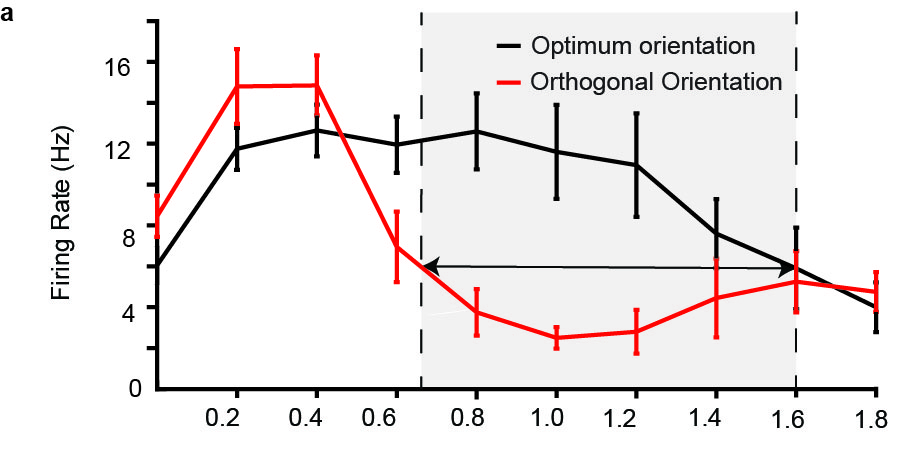
\includegraphics[width=\linewidth]{superiorcolliculus/SCOptOrth.jpg}
		\caption{Example SF tuning curves for optimum (blue) and
			orthogonal (red) orientations. The cut-off frequency at the optimal
			orientation is the SF at which the response at optimal orientation is no
			longer significantly different from the response at orthogonal
			orientation. The response at the cut-off frequency for optimum
			orientation is called the minimum response. For the orthogonal
			orientation, the cut-off frequency was the SF at which minimum response
			was first reached. Error bars are 95\% confidence intervals.}
		\label{fig:scoptorth}
		\end{figure}
	
Circular variance of the neurons at each spatial frequency was also
calculated using Equation 1 where spatial frequency tuning data for at
least four different orientations was recorded. The orientation
selectivity index (OSI) at each spatial frequency was also calculated as
1- reciprocal of orientation bias (Equation 2). The OSI instead of the
bias was calculated in this instance as 1) no comparison to previous
studies were made using this data; 2) The value of OSI would always be
within 0 and 1 whereas the maximum value of bias could be infinity; and
3) As this calculation only requires the spatial frequency data at the
optimum orientation and orthogonal orientations, a more complete data
set to examine the relationship between orientation tuning and the
spatial frequency tuning was present. The relationship between the OSI
and CV were also examined in the results.

	
	\subsubsection{Histology}
The brain that was stored in the sucrose at the end of the experiment,
was cut into 50 micron sections using a cryostat and then mounted on
gelatinised slides. The sections were then stained using Cresyl Violet
acetate solution. Lesions were identified and the electrode tracks
reconstructed using Adobe Illustrator to verify that all our neurons
were indeed recorded from the superior colliculus.
	
	\section{Results}
	
A total of 22 units were recorded from five tracks in three
anaesthetised Tree Shrews (2 female and 1 male). All neurons were from
the superficial layers of the SC. Of the 22 neurons, 20 were biased for
orientation. Spatial frequency tuning information was collected for 16
units, 12 of which showed low pass spatial frequency tuning. 13 of the
16 neurons also showed sharper orientation tuning at higher spatial
frequencies.
	
	
	\subsubsection{Anatomical location of units}
	
	The laminar position of all the units was determined by reconstructing
	the electrode tracks from the electrolytic lesions. The photomicrograph
	of a Nissl stained section from the SC is presented in figure 2a. The
	laminar position of the neurons determined from the electrode track
	reconstructions is shown in Figure 2b. All the recorded neurons were
	from the superficial layers, with the majority from the
	SGS.
		
	\begin{figure}[H]
		
		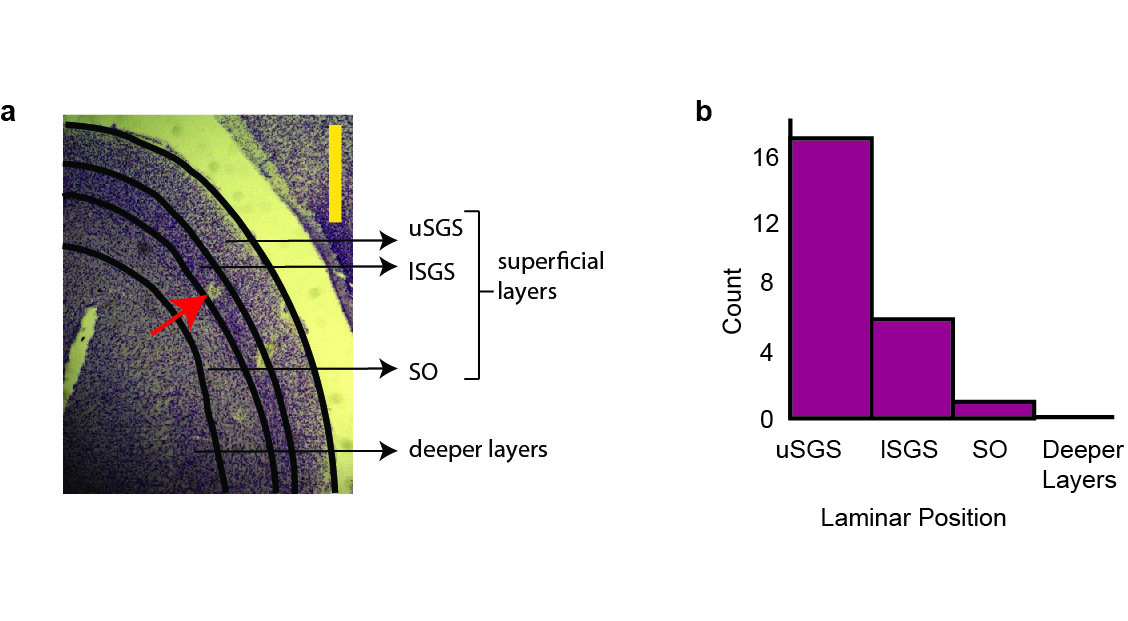
\includegraphics[width=\linewidth]{superiorcolliculus/anatpos.jpg}
		\caption{Laminar position of the neurons. (a) A photomicrograph of a tree shrew superior colliculus from the right hemisphere showing the different subdivisions of the superficial layers. The red arrow points to a lesion. Two other lesions from a different track are visible to the right of the lesion. The yellow scale bar is 1mm. (b) Number of cells sampled from each layer. Majority of the cells were from uSGS. Abbreviations: uSGS- upper Stratum Griseum Superficiale; lSGS- lower Stratum Griseum Superficiale; SO- Stratum Opticum.}
		\label{fig:anatpos}
	\end{figure}
	
	
	
	\subsubsection{Orientation Selectivity using bars}
	

The distribution of two measures of orientation selectivity are shown in
Figure \ref{fig:orihist}. Figure \ref{fig:orihist}a shows the distribution of circular variances. The
median circular variance for the sample was 0.80 (95\% confidence
interval(CI)= {[}0.70, 0.82{]}). The orientation tuning curves of a
representative neuron as well as those of the most selective, least
selective neuron with CV less than 0.9 and the least selective neuron in
the entire sample are presented in figure \ref{fig:range}a and b.

	\begin{figure}[]
	
	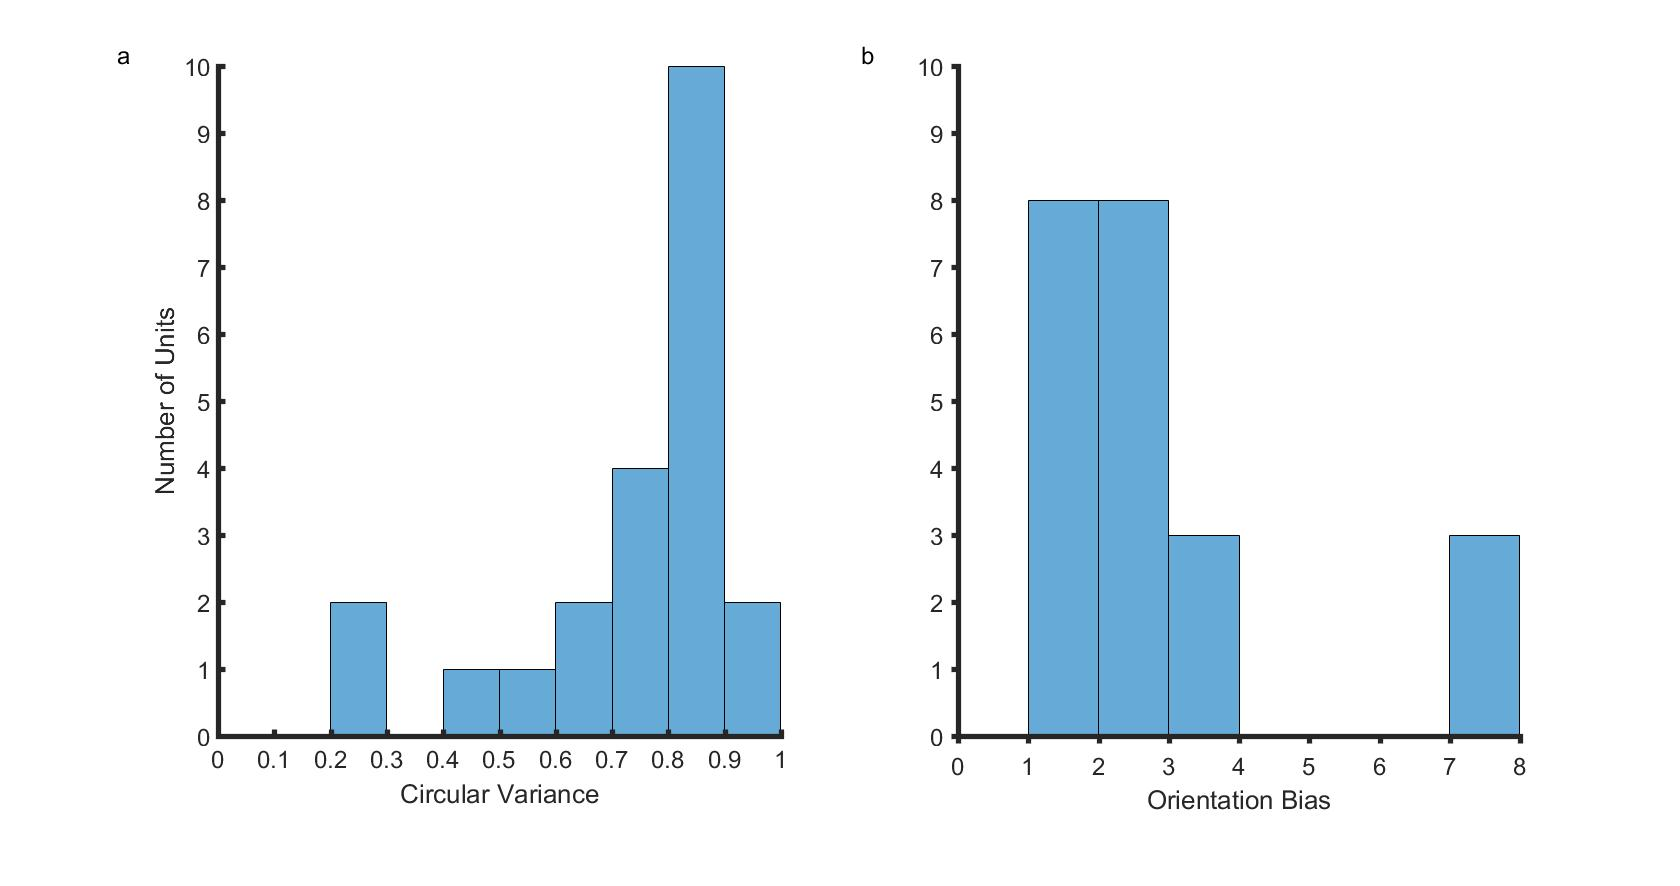
\includegraphics[width=\linewidth]{superiorcolliculus/orituning_fig.jpg}
	\caption{Orientation selectivity of neurons (a) This
		figure shows the distribution of circular variances of all neurons. (b)
		This figure shows the distribution of orientation biases.}
	\label{fig:orihist}
\end{figure}


\begin{figure}[]
	\includegraphics[width=\linewidth]{superiorcolliculus/cv.jpg}
	\caption{Orientation selectivity when measured with bars. (a) The
		orientation tuning of a representative neuron. The direction of movement
		of the bars are shown at the poles of the plot. The number next to the
		plot is the circular variance. The maximum firing rate of the neuron was
		117 spks/s. (b) Orientation selectivity of the sharpest, least tuned
		neuron included for further analysis and the least tuned neuron in the
		entire sample. The direction of movement of the bar are similar to (a).
		The circular variance of each neuron is displayed below. Maximum firing
		rate for the three neurons are 18 spks/s, 57 spks/s and 89 spks/s
		respectively. The response shown is the average of 10 trials and the
		error bars are ± 2*SEM. (c) the distribution of circular variances of
		all neurons in relation to the laminar position of the neuron.}
	\label{fig:range}			
\end{figure}

Any neuron with CV greater than 0.9 was classified as not selective to
orientation. Two neurons had a CV greater than 0.9 and hence were not
further recorded from.

An additional measure of orientation selectivity, the orientation bias
(Bias; figure \ref{fig:orihist}b) was also calculated. The median bias was 2.31 (95\%
CI={[}1.85, 3.20{]}). A bias of one would indicate that the response of
the neuron at the optimum and orthogonal orientations were the same.
Therefore, lower values of bias indicated that the neurons were more
broadly tuned. The two neurons that had circular variances greater than
0.9 had bias values closer to 1 (1.16 and 1.26). The orientation bias
was calculated to enable comparison with previous studies and further
analysis was not conducted using these values.

We also examined if there were any laminar differences in the
orientation biases, the circular variance of the neurons were also
plotted against the laminar position in figure \ref{fig:range}c. The neurons that
showed the sharpest orientation tuning were all located in the uSGS.	
	

	
	
	\subsubsection{Direction selectivity of neurons}
The distribution of the DSI and the DCV of 22 neurons are shown in
Figure \ref{fig:ds}a and b. All 22 neurons were included in the analysis as neurons
that are not tuned to orientation can be tuned to direction. Figure \ref{fig:dseg}a
shows a neuron that is selective to both orientation and direction. \ref{fig:dseg}b
shows a neuron selective to direction but not to orientation. The median
DSI was 0.69 (95\% CI= {[}0.5, 0.83{]}), suggesting that the majority of
the neurons were not direction selective. Of the 22 neurons that were
recorded from, only 5 (\textasciitilde{}20\%) satisfied our criteria for
direction selective neurons. The distribution of the DCV is shown in
figure \ref{fig:ds}b. The median DCV was 0.90 (95\% CI= {[}0.85, 0.93{]}). The DCV
was a more conservative measure of direction selectivity and none of the
neurons we measured from were selective to direction using this measure.
	
	\begin{figure}[H]
		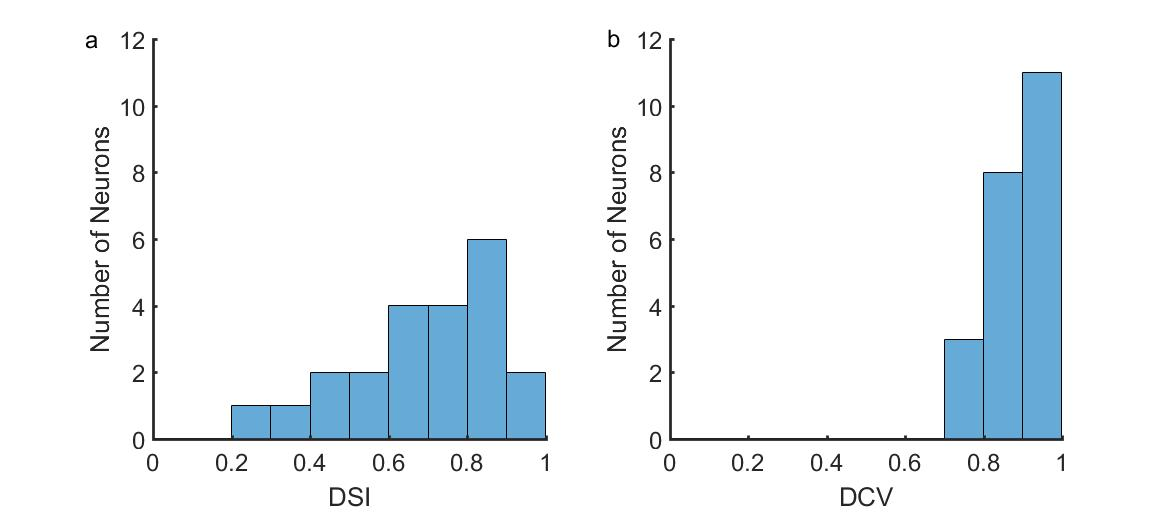
\includegraphics[width=\linewidth]{superiorcolliculus/directionselectivity_fig.jpg}
		\caption{Distribution of direction selectivity index of 22
				superior colliculus neurons using two different measures: the DSI (a)
				and the DCV(b).}
		\label{fig:ds}			
	\end{figure}
	
	\begin{figure}[H]
		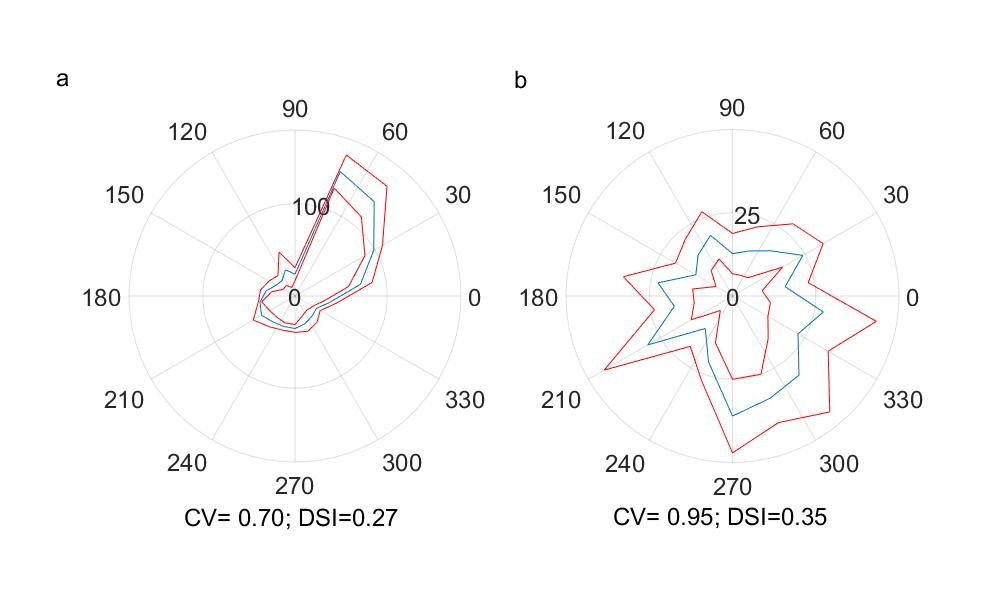
\includegraphics[width=\linewidth]{superiorcolliculus/Directionselectivity.jpg}
		\caption{Example of a cell that is selective to both direction
			and orientation (a) and a cell that is selective to direction but not
			orientation (b)}
		\label{fig:dseg}			
	\end{figure}
	
	\subsubsection{Spatial Frequency Tuning}
	
A summary of the results of spatial frequency tuning we obtained from 16
neurons is presented in figure 7a. The results from the LGN from Van
Hooser et al., 2013, Figure 7b, 30 neurons) were plotted on similar axes
in figure 7b to aid direct comparison. The median peak spatial frequency
of the SC neurons was 0.2 cpd (95\% CI= [0, 0.2]) and the median
half width at half height was 0.35 cpd (95\% CI= [0.15, 0.55]). SC
neurons tended to have higher spatial frequency cut-offs when compared
to the LGN neurons (figure 7b). A similar proportion of SC (80\%) and
LGN (76\%) neurons were low-pass tuned to spatial frequency .
	
	\begin{figure}[]
		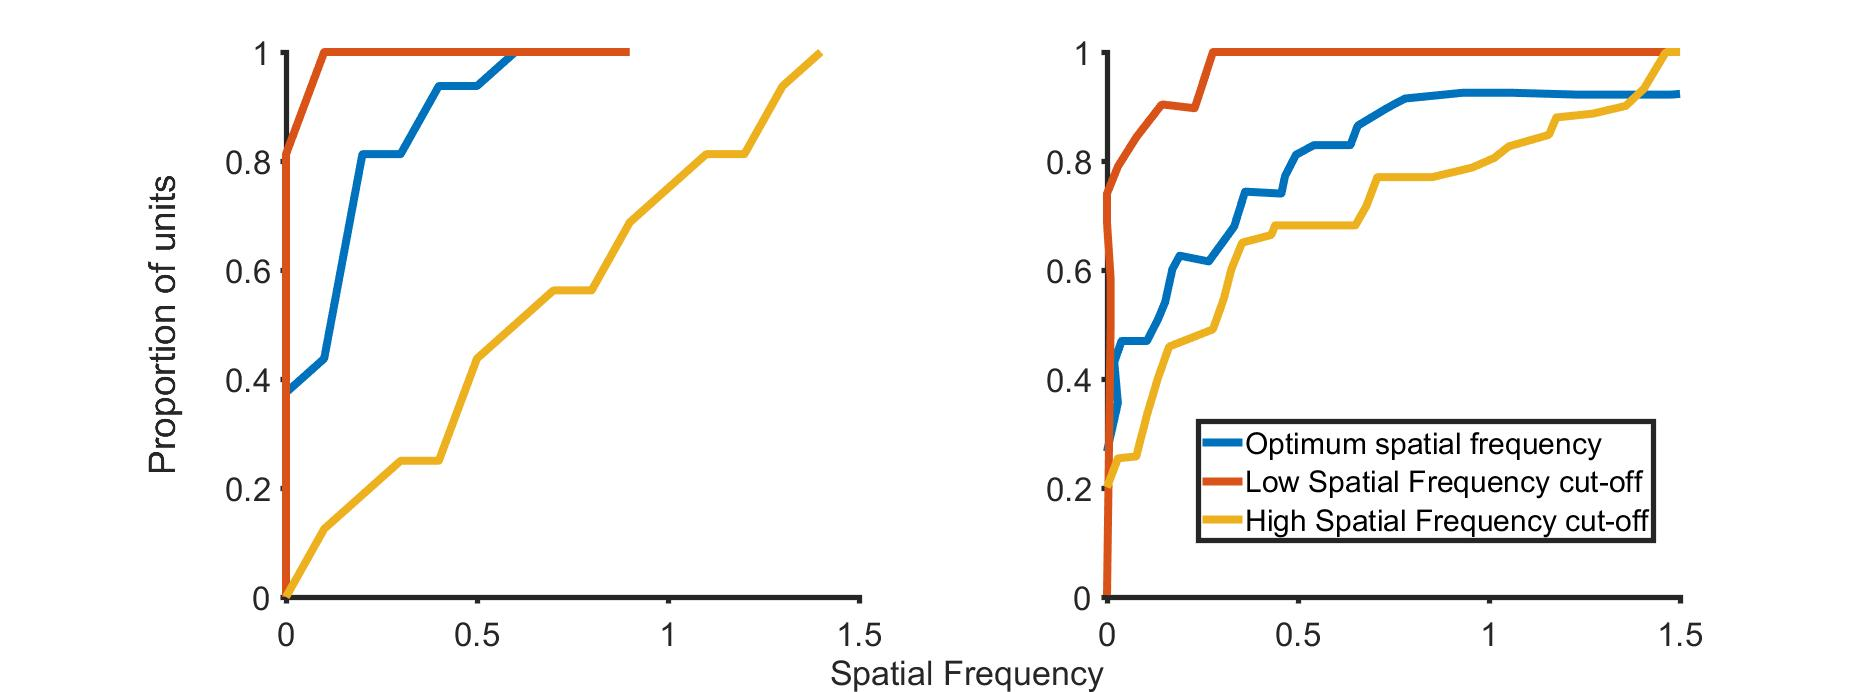
\includegraphics[width=\linewidth]{superiorcolliculus/cumsum_sf_SC_LGN.jpg}
		\caption{Cumulative distribution of the low-cutoff,
			optimum and high cut off spatial frequencies in the tree shrew Superior
			Colliculus for 16 neurons (a) and the Lateral Geniculate Nucleus for 30
			neurons (b; LGN). The LGN results were published in the paper by Van
			Hooser et al., 2013 (figure 7b) and plotted on the same scale as the SC
			data in the left hand side panel.}
		\label{fig:sfcumdist}			
	\end{figure}
	
	
	\subsubsection{Orientation tuning using gratings}
	
The circular variance of the orientation response of eleven neurons was
calculated at the peak spatial frequency and compared with those of
previously published data in the geniculostriate system of the tree
shrews. The distribution of these circular variances are shown in figure
8. The median CV of SC neurons when measured using gratings was 0.84
(95\% CI= {[}0.77 0.91{]}). The distribution of the CVs of the superior
colliculus and the LGN were similar. While in the LGN nearly 50\% were
not tuned to orientation at the peak spatial frequency, only 30\% of the
SC neurons did not show orientation tuning (1-CV\textless{}0.1). None of
the neurons demonstrated sharp orientation tuning (1-CV\textgreater{}
0.5) as observed in layer 2/3 of the cortex.
		
	\begin{figure}[]
		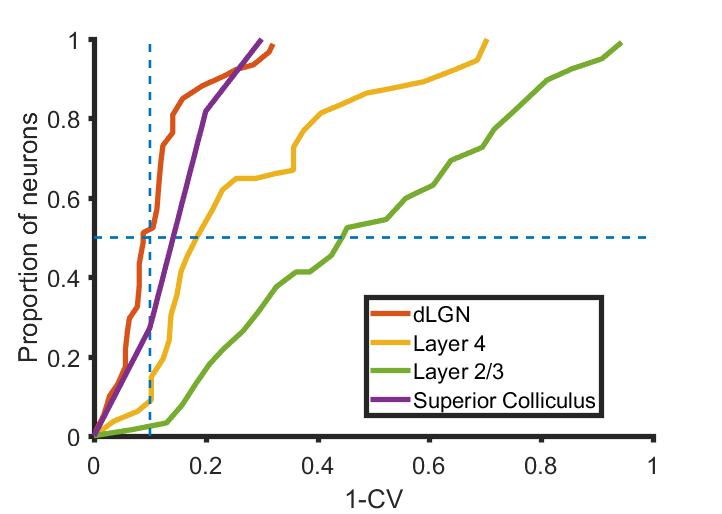
\includegraphics[width=\linewidth]{superiorcolliculus/orientation_bias_SG_geniculostriate_2.jpg}
		\caption{ Comparison of the distribution of the orientation
			selectivity of the LGN, Layer 4 and Layer 2/3 neurons to the
			distribution of orientation selectivity of the superior colliculus
			neurons. Horizontal dotted line indicates the 50\% of neurons and the
			vertical dotted line is the orientation tuning cut off.}
		\label{fig:CVvanhooser}			
	\end{figure}
	
As there was only enough data in 11 neurons to enable circular variance
calculations, the orientation selectivity index (OSI) was calculated for
the 16 neurons, where gratings of both optimum and orthogonal
orientation were calculated. The relationship of the OSI and the CV for
the 11 neurons where both these data were available is shown in figure \ref{fig:CVvOSI}. 
	
		\begin{figure}[]
		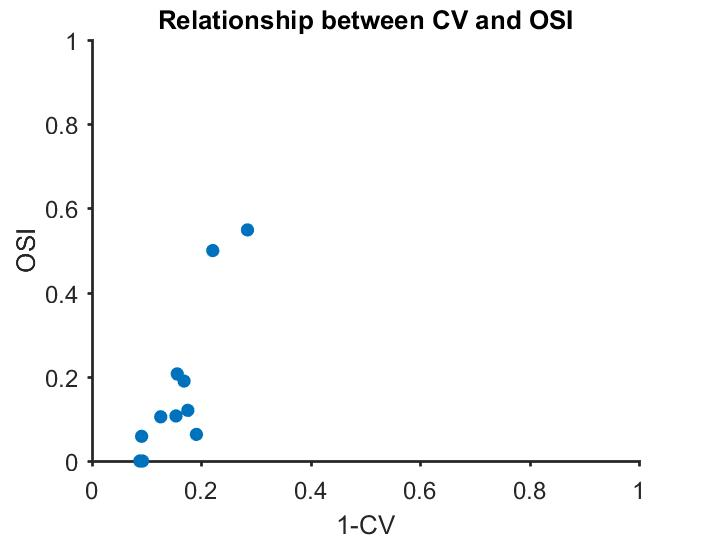
\includegraphics[width=\linewidth]{superiorcolliculus/CVvsOSI.jpg}
		\caption{Relationship between the circular variance and
			orientation selectivity index}
		\label{fig:CVvOSI}			
	\end{figure}
	
	Levick and Thibos (1982) calculated the circular variance of the neurons
	in their study at different spatial frequencies and found that neurons
	showed sharper tuning at spatial frequencies higher than the optimum
	spatial frequency. Since the circular variance and orientation
	selectivity index show a strong correlation (r= 0.87, p\textless{}0.005,
	n=11), in this chapter, OSI was used to conduct a similar analysis.
	
	\subsubsection{Relationship between spatial frequency and orientation tuning.}
	When the spatial frequency tuning response of the neuron at different
	orientations was measured, 13 of 16 neurons were tuned to orientation at
	higher spatial frequencies. The F0 components of a neuron's response to
	gratings of increasing spatial frequencies at the optimum and the
	orthogonal orientations are shown in figure \ref{fig:scoptorth}. The gray shaded area
	represents the spatial frequencies where the neuron still responds to
	gratings of the optimum orientation but no longer responds when gratings
	of the orthogonal orientation are presented (i.e., the neuron is
	orientation tuned). The difference in response between the optimum and
	non-optimum orientation cut off frequencies was calculated. These
	results for the group are presented in figure \ref{fig:sf_bw}. A one tailed Wilcoxon
	Signed Rank test showed that the spatial frequency cutoff at the optimum
	orientation was significantly higher than the spatial frequency cutoff
	at the orthogonal orientation (median difference= 0.4 cpd; z=3.15;
	p=0.0008). The magenta circles in figure 10 show the peak spatial
	frequency of the respective neuron and the green circles, the spatial
	frequency where the neuron was most tuned to orientation (where the OSI
	was maximum). The spatial frequency where the orientation tuning of the
	neuron was greatest was significantly higher than the peak spatial
	frequency of the neuron (One-tail Wilcoxon Signed Rank test; z=3.3096;
	p=0.0005), indicating that orientation tuning was observed at higher
	spatial frequencies in the tree shrew SC.
	
		\begin{figure}[H]
		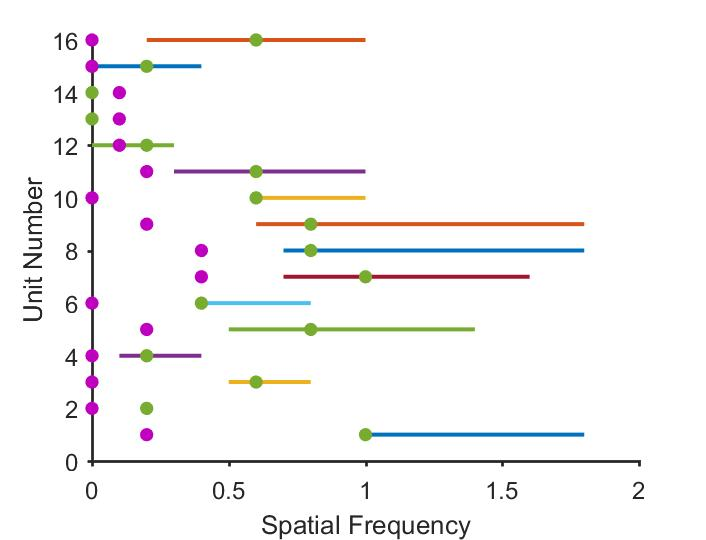
\includegraphics[width=\linewidth]{superiorcolliculus/sf_bandwidth.jpg}
		\caption{The difference between the cut-off frequencies
			for the optimum and orthogonal orientations for 16 units is shown in the
			above figure. The purple circles are the peak spatial frequencies of the
			respective neurons and the green circles are the spatial frequency where
			the cell is most tuned to orientation. In most cases, the neurons are
			most tuned for orientation at spatial frequencies well past the peak
			spatial frequency.}
		\label{fig:sf_bw}			
		\end{figure}
	
	\subsubsection{Modulation Index of the neurons.}
	
For the 16 units whose spatial frequency tuning were recorded, the
distribution of modulation ratios is presented in figure 11. A
modulation ratio less than one means that the modulated component of the
response was lower than the unmodulated component (non-linear cells)
while a modulation ratio of greater than 1 indicates that the neurons
were linear. The median value of the modulation index was 0.76 (95\% CI=
{[}0.65, 1.03{]}) suggesting that most neurons in our sample showed
non-linear summation over their receptive fields.
	
	\begin{figure}[H]
		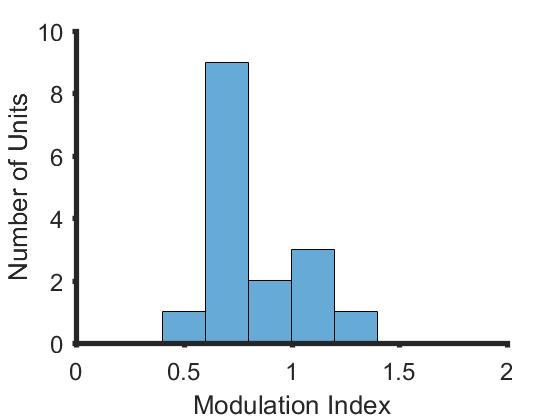
\includegraphics[width=\linewidth]{superiorcolliculus/modulation_index.jpg}
		\caption{The distribution of modulation indices of the
			neurons in our sample. Most neurons had a modulation index less than 1.}
		\label{fig:sc_mi}			
	\end{figure}
	\pagebreak
	\section{Discussion}
Our results show that the majority of neurons in the superficial layers
of the tree shrew SC show orientation biases when tested with bar
stimuli. When tested using grating stimuli, most neurons also showed low
pass spatial frequency tuning and demonstrated orientation tuning at
higher spatial frequencies. We also found that a small proportion of
neurons were tuned to direction and the majority of neurons showed
non-linear summation over their receptive fields.

We used bars to study the orientation selectivity of neurons in the
superior colliculus and found that most units (90\%) were biased for
orientation. We calculated two measures of orientation selectivity the
circular variance and bias. Neurons with a bias greater than or equal to
3 were comparable to the elongated receptive field units previously
reported (Albano et al., 1978). Six out of twenty-two neurons (27 \%)
had a bias greater than 3. This is comparable to the proportion of
elongated receptive field units (19\%) that were reported by Albano et
al (1978). Most of the elongated receptive field units reported by
Albano et al (1978) were found in the lSGS and SO layers and none were
recorded from the uSGS. In our sample, most neurons were biased for
orientation to some degree and neurons that had a bias greater than 3
were found in both the upper and lower SGS with the sharpest tuned
neurons found in the uSGS. We only recorded from one neuron in the SO
which had a bias value of 2.85. This discrepancy in the detection of
orientation biased neurons in the uSGS may be due to the thickness of
the bar stimulus used.

Neurons in the subcortical areas show more tuned responses when shown
thinner bars and at higher spatial frequencies (Vidyasagar and Urbas,
1982; Levick \& Thibos, 1980; Levick \& Thibos, 1982). In response to
gratings, at the peak spatial frequency, the SC neurons showed minimal
orientation biases and the orientation tuning of neurons were usually
more evident at higher spatial frequencies. As a result, if Albano and
colleagues used thicker bars than we have, they may have failed to find
neurons that had elongated receptive fields in the uSGS.

When the spatial frequency tuning of SC neurons and the LGN neurons in
the tree shrew were compared, both LGN and SC neurons showed low pass
spatial frequency tuning. However, when compared to the LGN neurons (as
published in Van Hooser et al., 2013), the peak spatial frequencies we
observed were lower. This could be related to the type of neurons the SC
neurons get their inputs from. SC neurons in most species receive inputs
from achromatic Y-like or W-like cells (DeMonasterio, 1978; Shapley \&
Perry, 1986; Schiller \& Malpeli, 1977; Bunt et al., 1975; Leventhal et
al., 1981). These cells show non-linear summation over their receptive
fields and tend to have lower peak spatial frequencies (Enroth-Cugell \&
Robson, 1966; Derrington \& Fuchs, 1979; So \& Shapley, 1981). Our
results indicate that the SC neurons show non-linear summation (as Y and
W cells do) over their receptive fields while the LGN neurons tended to
show more modulated responses, typical of X-like neurons (Van Hooser et
al., 2013). This could explain the difference in the peak spatial
frequency of the neurons from the two sub-regiongs. One other difference
between the LGN and the SC spatial frequency tuning curves was the high
spatial frequency cut-offs. The SC neurons generally tended to have
higher spatial frequency cut-offs compared to the LGN neurons. A
possible reason could be that in our study, we carefully tested the
responses of the neurons to stimuli of different spatial frequencies to
ensure that the neurons could resolve gratings of higher spatial
frequencies. If uncorrected refractive errors were present in the tree
shrews in the study by Van Hooser and colleagues, then this could
explain the difference in the high cut-off values reported between the
LGN and the SC.

Most neurons in the tree shrew superior colliculus were not tuned to
direction. Van Hooser et al reported that only one neuron in their
entire sample was tuned to direction using DCV in the geniculo-striate
system of tree shrews. Using the same measure, we found that none of our
neurons exhibited direction selectivity. A larger sample may show a
small proportion of neurons being tuned for direction using the DCV in
the superior colliculus. In their study, Albano and colleagues reported
that a proportion of the elongated receptive field cells were also
selective to direction of movement and that these cells were found in
the lSGS and the SO. However, the proportion of neurons tuned to
direction was not reported. Using a less conservative measure than the
DCV, the DSI, we found that approximately 20\% of the neurons were tuned
to direction. Of the 5 direction selective neurons, 2 were from the uSGS
(13\% of the uSGS neurons) and 3 were from the lSGS (50\% of the lSGS
neuons) suggesting that direction selective neurons were sparser in the
uSGS when compared to the lSGS.

In their study, Albano et al., (1978) proposed that the uSGS and the
lSGS could play different functional roles. They found that the uSGS
neurons were composed of only one type of neuron (the stationary
--responsive type) while the lSGS consisted of a combination of
different type of neurons. This claim was supported by anatomical and
morphological evidence; namely, uSGS neurons were generally smaller (5-8
μm) and received predominantly retinal inputs and lSGS neurons were
larger (8-12 μm) and received inputs from both the retina and the cortex
(Abplanalp, 1971). A later study however showed that the retinal inputs
dominated the SGS of the tree shrews with the uSGS receiving less
cortical inputs than the lower SGS. (Graham \& Casagrande, 1980). We
found that the uSGS contained the sharpest tuned neurons in our sample
and a smaller proportion of these neurons were tuned to direction
whereas, all the neurons in the lSGS were broadly tuned to orientation
and a higher proportion of neurons were tuned to direction. When
compared to Albano et al., we found more diverse response properties in
the uSGS rather than the lSGS (e.g.: see figure 4c). However, our sample
size in the lSGS was small (6 uSGS neurons) and any lack of diversity in
the neuronal responses could be attributed to sampling errors.

In this study we found that neurons in the superior colliculus were
tuned to orientation at higher spatial frequencies. Most neurons were
low pass tuned to spatial frequency and at the peak spatial frequency, a
similar proportion of neurons were biased for orientation in the LGN as
well as the SC. In the SC, neurons were sharply tuned to orientation at
higher spatial frequencies. This result is consistent with that observed
in the retina and the LGN of cats and macaques. Layer 4 neurons of the
tree shrews, which resemble LGN neurons (Van Hooser et al., 2013), also
respond similarly at higher spatial frequencies (See Chapter 5). This
similarity in subcortical orientation response across both the
geniculo-striate system as well as the SC indicate that orientation
biases observed in the LGN and the SC could be inherited from the
retina. In the tree shrew then, sharp orientation tuning observed in the
supra-granular layers could be due to the sharpening of orientation
biases by intra-cortical inhibition rather than through Hubel and Wiesel
like excitatory convergence.
	